\documentclass[conference]{IEEEtran}
\IEEEoverridecommandlockouts
% The preceding line is only needed to identify funding in the first footnote. If that is unneeded, please comment it out.
\usepackage{cite}
\usepackage{amsmath,amssymb,amsfonts}
\usepackage{algorithmic}
\usepackage{graphicx}
\usepackage{textcomp}
\usepackage{xcolor}
\def\BibTeX{{\rm B\kern-.05em{\sc i\kern-.025em b}\kern-.08em
    T\kern-.1667em\lower.7ex\hbox{E}\kern-.125emX}}
\begin{document}

\title{Ghost Town\\
{\footnotesize \textsuperscript{*}Note: Sub-titles are not captured in Xplore and
should not be used}
\thanks{Identify applicable funding agency here. If none, delete this.}
}

\author{\IEEEauthorblockN{1\textsuperscript{st} Selvia Andrew}
\IEEEauthorblockA{\textit{Department of Engineering} \\
\textit{name of organization (of Aff.)}\\
City, Country \\
email address}
\and
\IEEEauthorblockN{2\textsuperscript{nd} Jerry Guan}
\IEEEauthorblockA{\textit{Department of Engineering} \\
\textit{name of organization (of Aff.)}\\
City, Country \\
email address}
\and
\IEEEauthorblockN{3\textsuperscript{rd} Sean Wu}
\IEEEauthorblockA{\textit{Department of Engineering} \\
\textit{name of organization (of Aff.)}\\
San Jose, USA \\
shao-an.wu@sjsu.edu}
}

\maketitle
\thispagestyle{plain}
\pagestyle{plain}

\begin{abstract}
As we enter the era of data, online information becomes overwhelming, the recommender system has become an effective way to help users automatically select the information they need. Based on users’ browsing history, the recommendation engine can suggest user relevant items. However, in recent years, with deep learning being added to the recommender system, the recommendation algorithm became more precise and effective.The traditional recommender has been gradually replaced by deep learning based recommender system.
This article aims to provide a new technology in deep learning based recommender systems, called Generative Adversarial Network (GAN). We will discuss some of the commonly used recommender system technology including content-based, collaborative filtering and hybrid method, then, we will focus on how to apply GAN to recommender system to address data sparsity problem. Finally, we will expand on the current trend of recommender systems as well as the future challenges.
\end{abstract}

\section{Introduction}

Recommender system is an algorithm which aims to suggest user relevant items based on their browsing history[1]. During the last few decades, with the fast growing of e-commerce companies, the recommender system has been developed and widely used among most of the web sites, like Amazon, Walmart, eBay, etc[4]. Shopping from online retail stores like amazon or Walmart, users will get recommendations for other products based on their purchase records. Downloading music from Spotify or Pandora, songs either relevant to the singer or the genre will pop up. Watching videos on YouTube, the more videos the user watches, the more  accurate the recommender system will be. This is a win-win situation for both e-commerce companies and the users, the companies will sell more products, at the same time, users can find things close to their taste more easily without drowning into the overwhelming information.

It can be divided into three categories: collaborative filtering method, content-based filtering method and hybrid recommender system\cite{DL_overview}. Collaborative filtering is also called “user-item interaction matrix”, this method stores user’s past interactions with an item, such as the searching or purchase history, in a matrix, and then produces new recommendations solely based on this user-item matrix. Collaborative filtering could be divided into two subcategories: First is model based which usually uses machine learning method to produce a generative model which predicts the user’s future behavior using past use-item interaction record. Second is memory-based which uses the record of user history to make predictions, recently user search record is often used in this method. One of the main drawbacks of collaborative filtering is cold start, which means the sample dataset needs to be large enough for training models so that the model’s predictions are meaningful.

Unlike collaborative filtering which is based on user-item interaction, the content based recommender system is a method which relies on the product information. The information including both the user’s information like the age or sex and the item information like the type of a movie, the main actor, etc.. Since the content-based recommender system can only make recommendations based on existing interests of a user, the main problem of this method is the lack of variety of suggesting items. For a user who only has records on science fiction movies, the content-based recommender system won't be able to recommend any romantic movies to the user. 

The hybrid method is simply the mix of content-based and collaborative filtering. It combines various of inputs and/or composition of different mechanism. The benefit of this combination is that it can avoid the cold start problem. However, since the database is normally very large, the data of a single user only takes a tiny part of the total data. It will cause most of spot in user-item matrix left empty. This problem is called the data sparsity, because of insufficient data, the accuracy of recommender system will be decreased. Thus, it is important to have enough data before we conduct the recommender system. 

The Generative Adversarial Network(GAN) address the data sparsity problem well. The GAN model includes two parts, the first part is the generator, it generates the synthetic data based on existing data. The second part is the discriminator, which using classifier to identify the synthetic data. The closer the synthetic data to the real data, the better the GAN model. In this paper, we will discuss three GAN model based on the data accuracy. More concretely, we will talk about the implementation of these GAN model in detail. Finally, we will state the future developments and challenges of the recommender system. 

\section{Related Work}
Generative Adversarial Networks (GAN) were invented by Ian Goodfellow\cite{goodfellow_gan} and his colleagues in 2014 and it was introduced to deal with image data. GANs can be constructed in various ways. In the study of graph-base GAN recommender system, Xiaoyan Cai et al.(2018) integrate GAN into a unified framework to obtain efficient citation recommendation \cite{cai2018generative}. Pan et al.(2016) presented an graph-based academic paper recommendation approach using heterogeneous graph combined with other features\cite{pan2015academic}. IRGAN by Jun Wang et al.\cite{irgan}(2017) is the first time GAN being used in the information retrieval area. In Jun's studies, IRGAN provides a more efficient way of combining two types of information retrieval model. Jeayoon Yoo et al.(2017)\cite{yoo2017energy} proposed the energy-based GANs for recommendation system, by recasting the energy function, the energy-based GANs can be used as the instance of maximum-entropy imitation learning. 
This methods present in this paper is inspired by Homanga et al. (2018)\cite{RecGAN}, in their article, they combined Recurrent Neural Network (RNN) and Generative Adversarial Network (GAN) for a new model called Recurrent Generative Adversarial Network(RecGAN). This RecGAN model was evaluated using two dataset on MyFitnessPal and Netflix recommendation. As their study shows, the RecGAN can deal with the customer-GRU based RNNs as well as the current state-of-the-art models in a lot of evaluation metrics. As the result, the RMSE/RRN increased by 1.4\% using RecGAN.
In this article, we will introduce the TGAN for recommender system in the section below.

\section{Recommender System Overview}
\subsection{Content-based recommender system}
The concept of content-based recommender system is that it uses specific feature to build up user profile(a set of feature vectors), therefore the recommender system would be able to perform data mining procedure to gather similar profiles together and recommend one with each other. \\
\indent The architecture to build up a set of user profiles could be decomposed into several parts profiles\cite{Lops2011} such as Content Analyzer, Profile Leaner and Filtering Component. When a new entry comes in, it first goes through Content Analyzer for analyzing features and it was stored in Represented Items, then a feedback was created for the Represented Items repository.\\
\indent The biggest advantage for Content-based recommender system is that it does not need too much data on other users and is to recommend users with unique tastes without first-rater problem, lastly it could provide explanations with recommending insights. However the draw back of this method is that finding a good fit of features is hard, and to recommend items to new users is normally impossible as new users has no profile to begin with, and finally this method could be over specialized as it never recommends user with items that are even slightly off course as this could be a potential problem due to human's multiple tastes in heart. 

\subsection{Collaborative Filtering}

    1. concept\\
    2. development\\
    3. problem\\

\subsection{hybrid Method}

    1. concept\\
    2. development\\
    3. related work\\

\subsection{deep learning based recommender system}

    1. concept\\
    2. development\\
    3. related work\\



\section{Generated Adversarial Network}
\subsection{Synthetic Data Generation}
A primary purpose of this project is to generate a fake user browsing record that is similar to existing data. It is also important to keep the data distribution alike to the original data because of security reasons. Dissimilar distributions on synthetic data can give attackers potential insights that the data is synthetically generated. GANs can be constructed in various ways. Park et al. \cite{tableGAN} proposed to generate fake tabular data using Deep Convolutional GAN (DCGAN) \cite{DCGAN} that was originally developed for image data. Xu et al. \cite{TGAN} came up with the same idea of producing synthetic tabular data but using recurrent neural networks. After examining two different models, TGAN was selected for this project because of its ability to replicate the original data distribution.

\subsection{TGAN}
\subsubsection{Generator}
The TGAN's generator is built with Long Short-Term Memory (LSTM), a type of recurrent neural network architecture. According to the user-movie-record dataset, continuous variables in the dataset are rather uniformly distributed. Therefore, simple normalization on these features would not work properly because of their multi-modal distributions. Therefore, a Gaussian Mixture Model (GMM) is used to figure out where a certain feature belongs to one of Gaussian distributions with some probability. The authors of TGAN \cite{TGAN} used 5 Gaussian distributions. For discrete variables, the model uses a one-hot encoding and adds a noise, ranging from $0$ to $0.2$. Then, the sample is re-normalized. More detailed steps on how generator works within LSTM architecture is shown in Figure \ref{fig:tgan_structure}.
\subsubsection{Discriminator}
The discriminator uses $l$-layer fully connected neural network to distinguish real and fake data. It first concatenates outputs of LSTM cells (synthetically generated vectors). Within a mini-batch of samples, it calculates the distance of a sample to other samples in the mini-batch. At the end, it is able to determine whether a given data is fake or real. A brief diagram of a discriminator is also shown in Figure \ref{fig:tgan_structure}.

\begin{figure}[h]
\centering
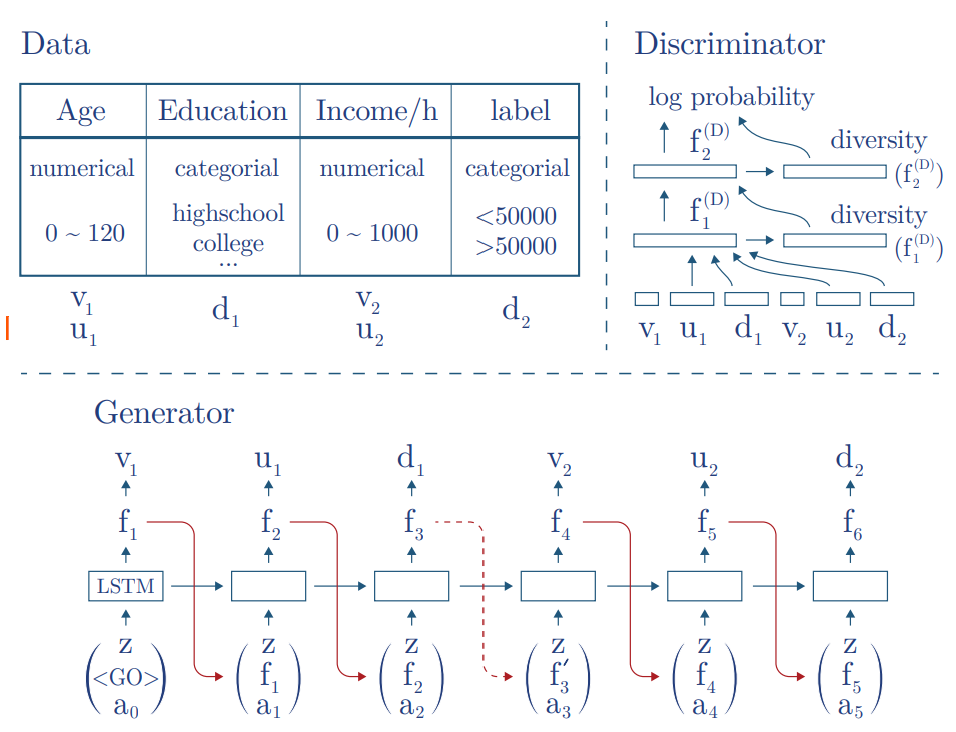
\includegraphics[width=\columnwidth, height=\textwidth, keepaspectratio]{graphics/tgan_structure.png}
\caption{An example of how TGAN's generator and discriminator plays a min-max game. Each continuous variable gets generated in 2 steps while individual discrete variable is generated in 1 step.}
\label{fig:tgan_structure}
\end{figure}

\section{Experiment}
\subsection{Generator Selection}
There are 3 different models that were trained to generate synthetic user browsing record. Each model has different hyper-parameters and input variables. Before going over the training part in more details, there are two representations of the original data. The first is a clean dataset where no scaling or normalization has been performed. The second representation has converted continuous variables into discrete variables by applying binning method. Only the last model uses the discretized data. After the individual model was trained, 1400 synthetic samples were generated. In order to match the total number of samples as the original, the last 15 rows were removed.

\subsubsection{Model I}
The first model was trained using 19 continuous variables and 10 discrete variables. With an Adam-optimizer, the training went with a learning rate of $0.001$ with 30 epochs where every epoch has 1000 steps. Many of other parameters were unchanged from the original training model.

\subsubsection{Model II}
The second model was also trained using 19 continuous variables and 10 discrete variables. With the same conditions like the previous model, we increased the duration of the training with 100 epochs and 500 steps per epoch. After training, we also generated 1385 fake samples and plotted to see the distribution. 

\subsubsection{Model III}
The last model was trained using the original data that was prepossessed by discretizing continuous variables into several bins.

\subsection{Discriminator Selection}
The purpose of a discriminator in this project is to test if the synthetic data is close enough to the authentic data. 
The selection process includes three steps. 
\begin{itemize}
\item First step is to choose an array of common classifiers and set the corresponding parameters. 
\item Second is to feed the model with training data and test its accuracy in test data set. 
\item Finally, we obtain the comparisons across the board and choose the best discriminator. 
\end{itemize}

\subsubsection{Discriminator Training}
To gain best accuracy, a list of classifier were used separately to fit the model, the classifier list includes: RandomForest with thirty(30) estimators, AdaBoost with thirty(30) estimators, Multi-layer Perceptron (MLP), K-Nearest Neighbors (KNN) with number of neighbors set from 10 to 60, Logistic regression, Gaussian Naive Bayes, Support Vector Machine. A pipeline was built so that we could train all of them in one cohesive procedure. In order to perfectly tune the parameters for each model, a leveraged grid search was used with a brute force search model. The parameters were preset as a list of choices and fed to the grid search function. To increase to training speed, we use dimension reduction to decrease the feed in data attributes of the raw data set. 

\subsubsection{Discriminator Selection}
The training-testing process is done in a cross validation manner. Specifically, a three-fold cross validation was implemented to reduce the effect of over-fitting. The results of accuracy scores of all the above-mentioned classifier is as below. Readers could also refer to the source code to learn about the detailed implementation of the model training pipeline process. 
After the training is done, the best model is used to predict on all of the authentic data to obtain an accuracy score on the entire data set. 

\subsection{Predicted Results}
Based on the different method in each GAN model, we can compare the results of three model by comparing the synthetic data generated by the these three model with authentic data. The ModelII works best with most similar distribution with original data. The best discriminator is the RandomForest classifier, combining the generator and discriminator, the accuracy reaches 98\%.

\section{Conclusion and Future Improvements}
In this work, we discussed the details of TGAN in recommender system.

\bibliographystyle{IEEEtran}
\bibliography{references}
\end{document}